\documentclass[aspectratio=169]{beamer}              % only frames

% for themes, etc.
\mode<presentation>
\usetheme{Madrid} 
\usecolortheme{crane}

%\usepackage{times}  % fonts are up to you
% The usual suspects
\usepackage{multirow, booktabs, dcolumn, color, graphicx} % Tables\usepackage{graphicx}
\usepackage{amsmath,amssymb,amsthm}
% Strikethrough text
\usepackage{soul}
% Adjust box to fit tabulars
\usepackage{adjustbox}
% Embed video
\usepackage{media9}
% For notes
\usepackage{pgfpages}
%\setbeameroption{hide notes} % Only slides
%\setbeameroption{show only notes} % Only notes
\setbeameroption{show notes on second screen=right} % Both
% Give a slight yellow tint to the notes page
%\setbeamertemplate{note page}{\pagecolor{yellow!5}\insertnote}\usepackage{palatino}
% Use colors by name
\usepackage{xcolor}
% EMBEDDING VIDEO IS POSSIBLE WITH PDFPC USE PDF PC to present
\usepackage{multimedia}



% The table highlighting for hypothesis discussion.
\usepackage[beamer,customcolors]{hf-tikz}
\usetikzlibrary{calc}

% To use background images
\newenvironment{colorframe}[2][]{%
\setbeamercolor{background canvas}{bg=#1}
\begin{frame}\color{white}}
{\end{frame}}


% To set the hypothesis highlighting boxes red.
\tikzset{hl/.style={
    set fill color=red!80!black!40,
    set border color=red!80!black,
  },
}

% Set Graphics folder
\graphicspath{{./figures/}}


% these will be used later in the title page
\title{Leaving Traces Online}
\subtitle{Using a VPN}
\author{Irfan Kanat}
\institute[CBS]{{Department of Digitization}\\ Copenhagen Business School}
\date{\today}



\begin{document}

% this prints title, author etc. info from above
\begin{frame}

	\titlepage

	\vfill
	{\tiny \centering This work is licensed under a \href{http://creativecommons.org/licenses/by/4.0/}{Creative Commons Attribution 4.0 International License}.}

\end{frame}

\note{In this module we will talk about what kind of traces we leave going about our daily lives and how to minimize this.}

\begin{frame}
	\frametitle{Not Using a VPN}
    
    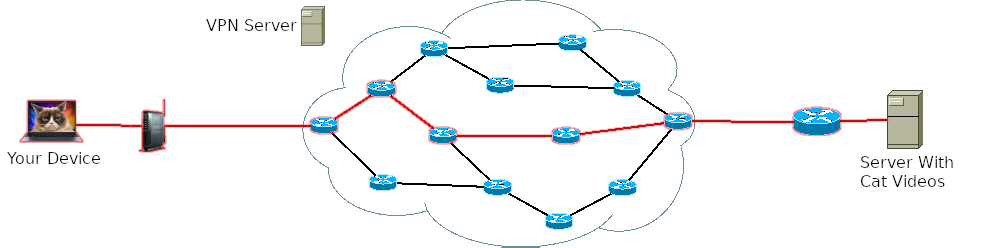
\includegraphics[width = \textwidth, height = .85\textheight, keepaspectratio]{figures/RoutingPathX.png}

\end{frame}

\note{Let's start with the typical internet use scenario.

When you don't use a VPN. Your traffic goes directly through all these routers between you and your target.

The connection may or may not be secured through encryption depending on the protocols used. Most HTTPs traffic today is encrypted, but other traffic such as DNS may not be encrypted.

Even if encryption is used, the operators of these routers will at least be able to link you to your device through the network addresses used in routing.
}

\begin{frame}
	\frametitle{Using a VPN as a Proxy}
    
    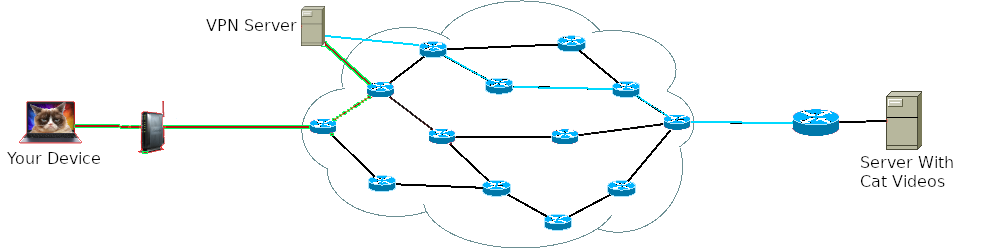
\includegraphics[width = \textwidth, height = .85\textheight, keepaspectratio]{figures/RoutingPathVPN.png}

\end{frame}

\note{When you use a VPN, ALL the traffic between you and the VPN server is encrypted (green outline). Thus its contents will be safe from snooping.

The routers along the red route with green outline will be able to link you to your connection to your VPN server. They will know you are exchanging encrypted data with the server, but they won't know what that data is.

The routers along the blue route will be able to see VPN server communicating with the target server. They may or may not be able to access the data exchanged (depending on the protocols). They likely won't be able to link you to this data or to the target server.
}

\begin{frame}
	\frametitle{Using a VPN as a Gateway}
    
    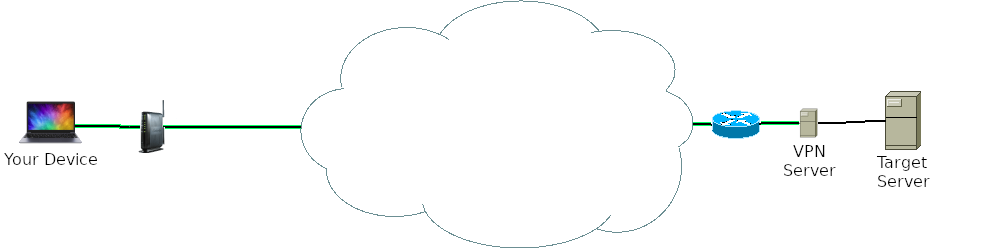
\includegraphics[width = \textwidth, height = .85\textheight, keepaspectratio]{figures/RoutingVPNGateway.png}

\end{frame}

\note{Another use case for VPN is using the VPN as a Gateway.

In this case VPN server acts as a bridge between your device and an organization's internal network.

Some CBS library resources for example are only accessible from within the CBS network. The VPN gateway allows you to act as if you were part of the CBS network.

The devices along the route won't be able to access any of your traffic as it is encrypted (green outline).
}

\begin{frame}
	\frametitle{Choosing a Trustworthy VPN Provider}
    \begin{enumerate}
    	\item Malicious VPN provider
    	\item Third parties accessing VPN logs
    	\item Governments accessing VPN logs
    \end{enumerate}

\end{frame}

\note{If you consider the role of a VPN provider, you would see the importance of trust in this relationship. All your traffic will route through their servers. 

First of all, you need to be able to trust that the VPN provider is a legitimate business and not some shady operation. Many free VPN providers have been known to inject adds and worse into VPN traffic. So I don't recommend you use one of these.

Secondly, you need to be able to trust that third parties won't be able to obtain VPN logs. Some VPN providers claim they don't keep any logs. So even if a third party legally requests these logs, they won't be able to access these.

Third, you don't want your VPN provider to roll over and hand out your data to foreign governments. So choose one that is not within their jurisdiction.}

\begin{frame}
	\frametitle{Using a VPN}
    
	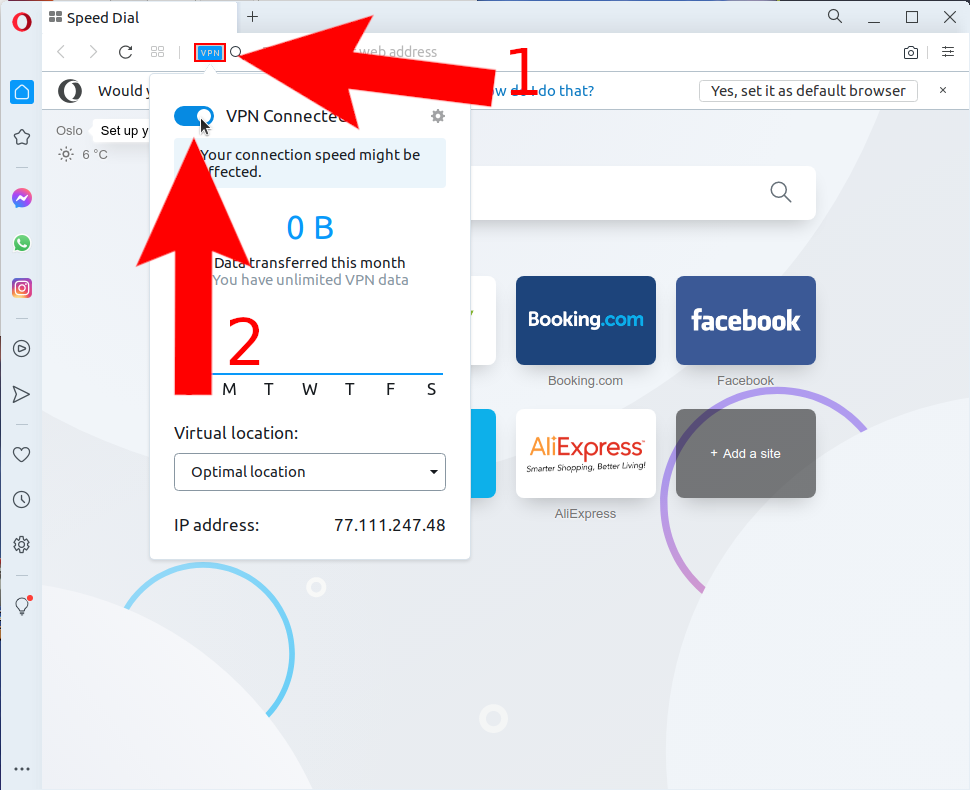
\includegraphics[width = \textwidth, height = .85\textheight, keepaspectratio]{figures/OperaVPN4.png}

\end{frame}

\note{I would normally recommend a real VPN service such as NORD VPN or Proton VPN. For this in class exercise however, we will use something that is conveniently available and free.

Opera web browser comes with a Free VPN. This means all your activities in the browser goes through Opera's VPN service.

It is not the best in terms of security or speed, but it is very easy to set up.

Other browser operators (Firefox/Mozilla) are also developing their own VPN solutions.}

\begin{frame}
	\frametitle{A Word of Caution About Opera VPN}

	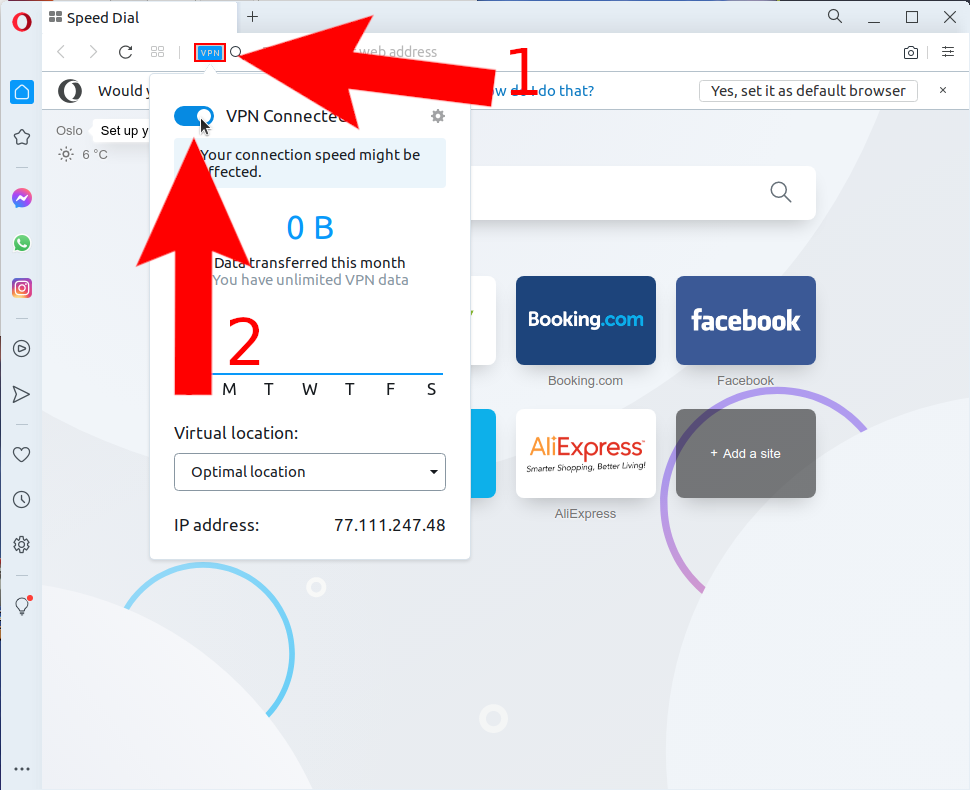
\includegraphics[width = \textwidth, height = .85\textheight, keepaspectratio]{figures/OperaVPN4.png}

\end{frame}


\end{document}
